\clearpage
\hypertarget{growBox tex}{}
\subsection{Implementing grow}
\texHeader

\vspace*{0.5cm}

\begin{itemize}

\item[$\blacktriangleright$] In \texttt{box.grow()}, create a simple control flow with one story pattern (Fig.~\ref{fig:growDecl}). 

\begin{figure}[htbp]
\begin{center}
  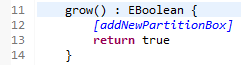
\includegraphics[width=0.4\textwidth]{eclipse_growDecl}
  \caption{Basic control flow to grow \texttt{box}}
  \label{fig:growDecl}
\end{center}
\end{figure}

\item[$\blacktriangleright$] Create and open the new pattern. You'll want it to match the invoking box with \emph{any} two partitions, so create a bound
\texttt{this} box, and the free variables \texttt{firstPartitionInBox} and \texttt{lastPartitionInBox}. You'll also need an object variable (set to create) to
represent the new partition. The skeleton of your pattern should now resemble (Fig.~\ref{fig:growPattSkel}).

\vspace{0.5cm}

\begin{figure}[htbp]
\begin{center}
  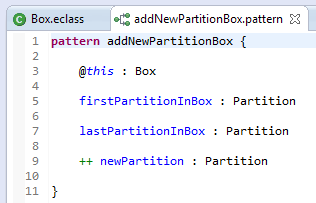
\includegraphics[width=0.5\textwidth]{eclipse_growPatternSkeleton}
  \caption{The \texttt{addNewPartitionBox} skeleton}
  \label{fig:growPattSkel}
\end{center}
\end{figure}

\item[$\blacktriangleright$] Next, we need to create an appropriate \emph{NAC} which will constrain the possible choices for \texttt{lastPartitionInBox}.
Create a negative \texttt{next\-Part\-it\-ion} object variable by using the negation `!' operator.

\vspace{0.5cm}

\item[$\blacktriangleright$] Now add \texttt{`->next : nextPartition'} to \texttt{lastPartition}'s scope. This attempts to establish a \texttt{next} link from
the last partition. Next, add \texttt{`++ ->next : newPartition'} (Fig.~\ref{fig:firstNAC}). This constraint will only be fulfilled if the NAC fails, and it
establishes the \texttt{newPartition} as the final partition.

\begin{figure}[htbp]
\begin{center}
  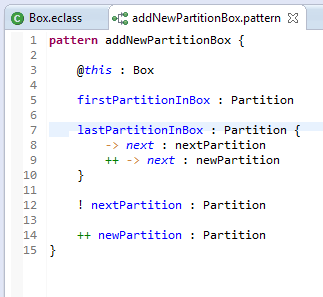
\includegraphics[width=0.5\textwidth]{eclipse_growLastNAC}
  \caption{Creating the first NAC \update}
  \label{fig:firstNAC}
\end{center}
\end{figure}

\vspace{0.5cm}

\item[$\blacktriangleright$] In a similar fashion, create a second NAC, \texttt{previousPartition}, for \texttt{firstPartitionInBox}. No new references have to
be created here, so all you need to establish is the link connecting \texttt{firstPartitionInBox} to the negative element, \texttt{previousPartition}
(Fig.~\ref{fig:growPatt}).

\begin{figure}[htp]
\begin{center}
  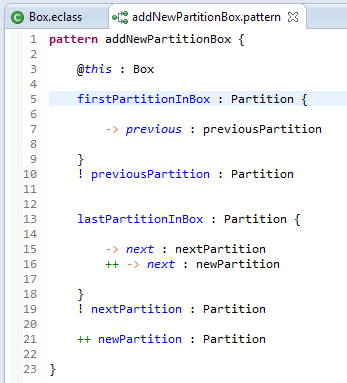
\includegraphics[width=0.55\textwidth]{eclipse_growFirstNAC}
  \caption{Pattern with both NACs}
  \label{fig:growPatt}
\end{center}
\end{figure}

\item[$\blacktriangleright$] Now edit \texttt{@this} with appropriate link variables to the first and last partitions. Try using auto-completion here for the
reference names!

\newpage

\item[$\blacktriangleright$] The next step is to establish the \texttt{box} and \texttt{previous} references in our newly created object variable,
\texttt{newPartition}. While you could of course write \texttt{`++ ->box : this'}, any link variables established here are automatically set to `green,' and do
not need to be explicitly set with an \texttt{++} operator. This is because you cannot connect a `black' link to a `green' node.\footnote{Remember that a rule
actually consists of two graphs: r = (L,R). A green node only belongs to R and not to L, while a black link is in L and in R. If the target of the link is only
in R, however, L would have a link with an undefined target. This is not allowed (L is not a graph).} In other words, a `green' object variable has a global
effect on all link variables declared in its scope.

\item[$\blacktriangleright$] Your pattern should now resemble Fig~\ref{fig:growAllLinks}. 

\begin{figure}[htp]
\begin{center}
  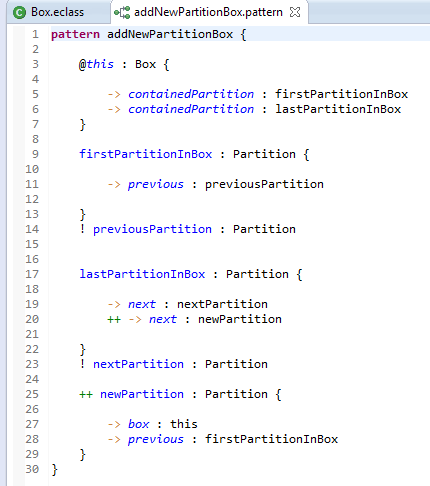
\includegraphics[width=0.65\textwidth]{eclipse_growLinks}
  \caption{Pattern  with deterministic choice of first and last partitions}
  \label{fig:growAllLinks}
\end{center}
\end{figure}

\item[$\blacktriangleright$] We're not \emph{quite} done yet - our newest partition doesn't yet have a size. This means that not only do we need to make
another attribute constraint to set its value, but \texttt{newPartition} needs to directly invoke a method in order to get the correct value. You can do this
via a \emph{MethodCallExpression}. The structure of this expression is similar to Java where:
\syntax{MethodCallExpression := (object\_variable\_expression | \\ parameter\_expression)`.'ID`('argument\_list `)'}

\item[$\blacktriangleright$] We've encountered both of these expression types already -- \texttt{`@'} in \texttt{removeCard} and \texttt{`\$'} in
\texttt{check}. The latter doesn't apply to this pattern, so write: \syntax{@this.determineNextSize()}.

\item[$\blacktriangleright$] Your workspace should now resemble Fig.~\ref{fig:patternComplete}.

\vspace{0.5cm}

\begin{figure}[htp]
\begin{center}
  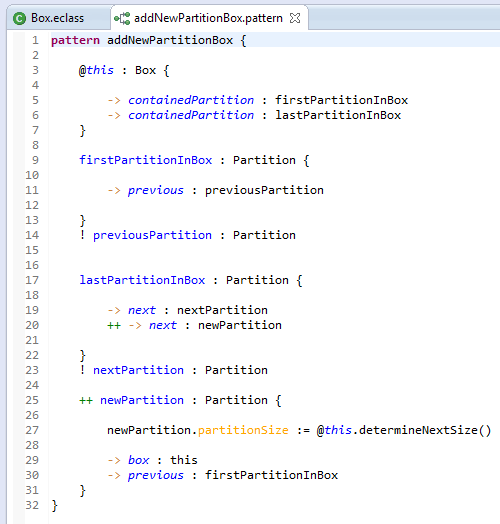
\includegraphics[width=0.9\textwidth]{eclipse_growFinished}
  \caption{Complete pattern for adding a new \texttt{partition} to \texttt{Box}}
  \label{fig:patternComplete}
\end{center}
\end{figure}

\vspace{0.5cm}

\item[$\blacktriangleright$] \emph{Now} we're done! While NACs may be difficult to understand at first, as you can see, they're not hard to implement, and
can be used in a wide variety of applications. To see how this method is implemented in the visual syntax, check out Fig.~\ref{fig:growComplete} in the
previous section.

\end{itemize}